\chapter{Implementation}

\section{Preparation of Data}
The mri files are 256 $\times$ 256 $\times$ 256 matrices but we are only interested in the small part which overlaps with the masks from segmentation, i.e. where the elements in segmentation is either 1 (left hippocampus) or 2 (right hippocampus).
We have created the function HippoMatrix, which takes three variables, which file to load, wether or not erosion should be performed, and if the left or right hippocampus is desired.
First we assign a value based on if we are looking for the right hippocampus, as they are associeated with 1 and 2 respectfully.
If erosion is desired we create the city-block for erosion by taking advantage of distances calculations, distance = $\sqrt{x^2+y^2+z^2}$. All parts of the city-block have distance 1 from the origin point. With the city-block defined we can use matlabs build in function imerode to perform the erosion. \fixme[inline]{insert snip of code.+ link imerode page}

Looping through the entiere segmentation matrix we identify all the datapoints where segmentation is one for the left hippocampus or two if we are trying to identify the right hippocampus. For each instance in segmentation we save the coordinate (i,j,k) and the mri(i,j,k) value in an array as v(1) = (i$_1$,j$_1$,k$_1$,mri(i$_1$,j$_1$,k$_1$)).\fixme[inline]{snip of main loop, explain left is also used incase of right}

On the basis of this we can create a three-dimensional matrix which contains all the datapoints, hippoBox = max(i) - min(i) + 1 $\times$ max(j) - min(j) +1 $\times$ maj(k) - min(k) + 1.
Then we simply loop through our array with the relevant data and input them into hippoBox, all other elements inside the matrix are set to NaN. \fixme[inline]{snip of last loop}

The return value from the function is the matrix hippoBox containing only the relevant data.

\section{Data Calculations}

In our function file, we do a lot of stuff that will be described in details. But in this file, we load our labels file, and take care of calculating every patient file to find a GLCM and from this GLCM we find the GLCM features.

First we check wether we have a patient with AD or not and name them respectively to their group.

Now we calculate the GLCM for the 2D and 3D which we have two function doing the work. These functions, \texttt{glcm2dFast} and \texttt{GLCM3D}, take the \texttt{HippoMatrix} data, as mentioned in preparation data, and the desired distance that we wish to calculate to.

Now we initiate two cells for the GLCM Features which we derivative using the function \texttt{GLCMDerivations} which will take the GLCM data and if we wish to normalize the GLCM or not as input.

\begin{lstlisting}[language=Matlab]
        data_glcm2D = glcm2dFast(HippoMatrix(files(j).name, erode, leftright), 10);
        data_glcm3D = GLCM3D(HippoMatrix(files(j).name, erode, leftright),10);

        data_Derivations2D = cell(90, 1);
        data_Derivations3D = cell(130, 1);

        for k = 1:size(data_Derivations2D, 1)
            data_Derivations2D{k} = GLCMDerivations(data_glcm2D{k}, norm);
        end
        for k = 1:size(data_Derivations3D, 1)
            data_Derivations3D{k} = GLCMDerivations(data_glcm3D{k}, norm);
        end
\end{lstlisting}

Lastly we save the data to their respectively folders.

\subsection{Calculating GLCMs}

To calculate the GLCMs in two-dimensions we have taken advantage of matlabs built-in function graycomatrix. It calculates as described in methods. It is then a matter of giving the proper offsets, and the right number of GIs. We can then loop through the hippoBox slices and sum up the GLCMs.\fixme[inline]{snip af glcm2dallangels hvor vi udregner}

We ultimately save all 90 glcms in a cell.\fixme[inline]{Fodnote der beksriver hvad en cell er?}

To implement the three-dimensional GLCMs we have created our own function.
The function GLCM3D takes a hippoBox as data and how many distances desired. I then for each distance loop through the entire matrix, and for each element it chekcs if it is NaN value and larger than zero. The check utilizes that NaN is not larger than zero, so data(i,j,k) > 0 returns false incase of data(i,j,k) = NaN.
The reason we also insist that it should also be larger than zero is because a few of the right hippocampus include GI of value zero in their hippoBox, but as zero is the value the mri scans have outside the brain we choose to ignore the few instances. To include them would mean we had to increase our GLCMs by 1 in size, which would make them differ from the GLCMs derived in two-dimensions, making the comparison unfair. In addition matlab start their index for their matrices with one and not zero so we would also have to add every index with one creating greater complexity.
\fixme[inline]{snip af første if.}
Given that the datapoint is relevant, i.e. larger than zero, we then have to look at the thirteen offsets, to see if we need to increment an element in on of the GLCMs. For each offset check if the offset is inside the hippobox, and is the offset elemnt a non NaN nonzero value. If so we then increment the relevant GLCM, lets say it is the offset(d,0,0), d = 1, in element GLCM$_(d,0,0)$(x,y) (hippoBox(i,j,k),hippoBox(i+1,j,k)).
\fixme[inline]{indsæt en if statement}

We have defined our thirteen offsets as \{(d,0,0),(d,0,d),(0,0,d),(-d,0,d),(d,-d,0),(d,-d,d),(0,-d,d),(-d,-d,d),(-d,-d,0),(-d,-d,-d),(0,-d,-d),(d,-d,-d)(0,-d,0)\}.
Because of the relationship between the offsets, as in GLCM$_{(d,0,0)}$ = GLCM$_{(-d,0,0)}^T$, the results do not change depending of the dimensions as long as there are no offsets where offset$_i$ = offset$_j^T$ holds.
We calculate those thirteen offsets for distances one through ten, and save all 130 GLCMS in a cell.
\fixme[inline]{indsæt en if statement}

\section{Naive feature}
only done it 3D
Left Hippo
Features selected: 8
Imoc2: A7D2, A3D3, A13D3
Imoc1: A13D9, A7D6
Entro: A13D10, A7D6
SumAv: A7D6

\subsection{Calculating(Computing) the GLCM Features}

\fxnote[inline]{Snak om Datacalculation filen}

In the implementation of the GLCM Feature derivation we are taking two inputs. The first input variable is the GLCM matrix and the second is wether we wish to normalize the data.

What we are doing first is to make sure that all variables are implemented. Firstly we find the size of the GLCM which will be the greylevels. Hereafter we can initiate the $C_x$, $C_y$, $C_{x+y}$ and $C_{x-y}$ since we know the size of the GLCM.

For the pixel values in the GLCM we are using MATLAB's \texttt{ind2sub} function, that is a command that determines the equivalent subscript values corresponding to a single index into an array.\fxnote[inline]{Lav et eksempel (diagram) af hvordan cxminusy og cxplusy ser ud}. We are using these variables in the GLCM Features as seen in Appendix \ref{derivationfeatures}.

To calculate the $C_{x+y}$ and $C_{x-y}$ we have two for loops as seen in Appendix \ref{Cxplusy} and \ref{Cxminusy} where N of course is the greylevels. \fxnote[inline]{Snakke om optimeret altså filerne Cx+-y}

To find the mean and standard deviation for $C_x$ and $C_y$ we just use the functions that MATLAB have.

The GLCM features, as seen in Appendix \ref{derivationfeatures}, utilizes MATLABs use of vectorization. This is rewarding in the vectorized code appears more like the mathematical expressions and makes the code easier to understand and is shorter. There is often a performance gain in using vectorized code than the corresponding code containing loops.

It should be obvious for the reader to tell that the code looks alot like the mathematical expression like in Appendix \ref{derivationfeatures}.

\begin{lstlisting}[language=Matlab]
HXY1 = -nansum(glcm(tmpsub)'.*log(cX(I).*cY(J)));
HXY2 = -nansum(cX(I).*cY(J).*log(cX(I).*cY(J)));
HX   = -nansum(cX.*log(cX));
HY   = -nansum(cY.*log(cY));
HXY  = -nansum(glcm(:).*log(glcm(:)));

stats.angularSecondMoment                = sum(glcm(:).^2);
stats.contrast                           = sum(abs(I-J).^2.*glcm(tmpsub));
stats.correlation                        = (sum(I.*J.*glcm(tmpsub)) - muX*muY) ./ (stdX*stdY);
stats.variance                           = sum(((I - mean(glcm(:))).^2).*glcm(tmpsub));
stats.inverseDifferenceMoment            = sum(glcm(tmpsub)./(1 + (I-J).^2));
stats.sumAverage                         = sum(bsxfun(@times,(2:2*nGrayLevels)',cXplusY));
stats.sumVariance                        = sum(((2:2*nGrayLevels) - stats.sumAverage)'.^2.*cXplusY((2:2*nGrayLevels)-1,1));
stats.sumEntropy                         = nansum(cXplusY.*log(cXplusY));
stats.entropy                            = HXY;
stats.differenceVariance                 = var(cXminusY);
stats.differenceEntropy                  = nansum(cXminusY.*log(cXminusY));
stats.informationMeasuresOfCorrelation1  = (HXY - HXY1)./(max(HX,HY));
if (strcmp(norm, 'normalize') == 1)
    stats.informationMeasuresOfCorrelation2  = sqrt(1-exp(-2.*(HXY2 - HXY)));
else
    stats.informationMeasuresOfCorrelation2  = NaN;
end
\end{lstlisting}


As seen from line 19 to 23, we have an if-statement. This checks if we call our plot on the normalized data or not, since the values on \texttt{informationMeasuresOfCorrelation2} end up being $\pm \infty$ when the data are not normalized. \fxnote[inline]{Snakke om hvorfor normalized data. Features vi har valgt fra freebourug har gjort det og måske gjort i det mente om at de kan ende med pæne værdier -- i method muligvis}


\section{Plotting the GLCM features}
Now that we have calculated the 13 GLCM features, we can plot them. Remember that one GLCM matrix have one specific distance for a specific offset, so this equals 90 GLCMs for the 2D, after some cuts and 130 GLCMs for the 3D version. To plot, you would simply have to call the function \texttt{simpleAllplot} that takes 4 inputs, the \texttt{DATA} which are the GLCM data, \texttt{NumberOfPatients} i.e. how many patients we wish to plot, \texttt{looping} which tells the function how many features it should count on, counting from feature one and Lastly in the \texttt{simpleAllplot} function we give us self the possibility to chose between plotting the mean values, for a specific number of patients or both.

We have discussed how our plain data is sorted when \texttt{datacalculation}, now we wish to sort it differently for our plots, so it is easier to handle. Since we have 13 GLCM features  we create 13 cells to easier name our plots for the for loop sorting the data. The way we chose to sort our data is to have it in the following way \texttt{Dataset(NumberOfPatients*10, 9, 13)}. So we have 9 subplots per Feature where each subplot for every plot have distance 1 to 10 

\begin{figure}[H]
  \centering
  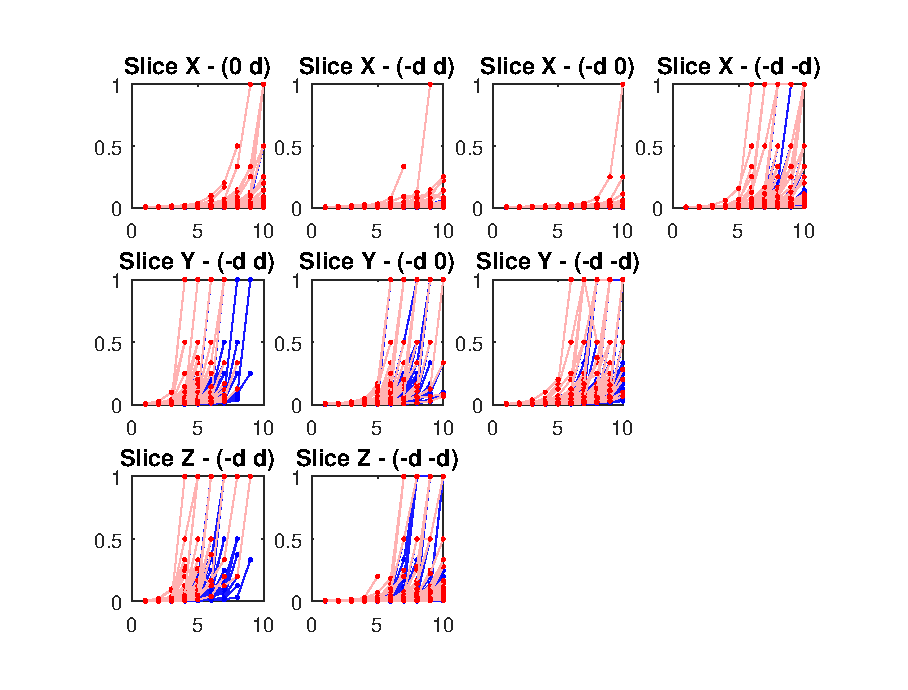
\includegraphics[scale=0.65]{ASMerode.eps}
  \caption{Plot of the Angular Second Moment features where the data have been normalized and eroded. The red are the patients with AD and the blue are the rest}\label{fig:ASMNormalizedEroded}
\end{figure}



\section{Forward feature selection}

We want to use cross validation on our feature selection. To do achieve this we need to create 10-folds for our patients, which means we have to randomize the order of the patients. We use Matlabs build in function datasample to randomize the data and the pick five Control patitens, followed by five AD, for each fold, which we continue until all 100 patients have been selected, leaving us with 10 folds with each five control and five AD.

To make the data easy to work with we sort it into a matrix, F = (No. of patients $\times$ No. of offsets $\times$ No. of GLCM features $\times$ No. of distances). It is not necessary to split the matrix up into one for each fold, it is easier just to remember the first ten are fold one, fold two are F(11-20, :, :, :), etc.

Firstly we wish to calculate how well each feature is at predicting on it its own. So we create a matrix, evaluate = (No. of offsets $\times$ No. of GLCM features $\times$ No. of distances). For the two-dimensional data evaluate is a 9 $\times$ 13  $\times$ 10, which is equal to 1170 different features for each patient, in three-dimensions we have 13 $\times$  13  $\times$  10 = 1690. This huge amount of features allow us to make a preliminary cursory feature elimination, where any feature that is not complete i.e. any feature that has a NaN value for one or more of the patients we choose to ignore. In practice this is done by setting their entry in evaluate to zero. The check for NaN is done with
\begin{lstlisting}[mathescape=true]
	if (~isempty(find(isnan(dataset(:,i,j,k)) == 1, 1)) == 1)
\end{lstlisting}
For the GLCM feature j calculated at offset i with distance k, it finds for all the time that value is NaN for all the patients, and checks if that set is an empty set. If the set is not empty it returns 0, which is negated and is equal to 1, so the if statement returns true and evaluate(i,j,k) = 0. We set it to zero as we evaluate each features over how well it predicts, and not how many missclassifications it makes. It is a trivial difference as 1 - succes = error.

The prediction of each feature is evaluated using the function knnWithCrossval. The function splits the data up into the appropriate sets and trains a knn for each training set. We use Matlabs fitcknn function to fit the model, with euclidean distance, standardized data and for k = 1,2,...,10. However we run the entire feature selection for each k seperately. The functions returns the averaged prediction score for the folds.
We then find the feature with the highest accuracy and for the next iteration of evaluations the selected data is used in the creation of the knn models in knnWithCrossval.
\begin{lstlisting}[mathescape=true]
    knnmodels{i} = fitcknn(horzcat(trainKfolds{i},chosenTrainKfolds{i}),label90,'Distance','euclidean',...
    'NumNeighbors',k,'Standardize',1);
\end{lstlisting}
Where horzcat is a horizontal concatenation of matrices.
If the best evaluation of the features is worse than if no new feature is selected the algorithm breaks, and returns a matrix of selected features and iterated accuracy, as well as the last best feature not to be selected.
Incase of ties for best feature we select the first entry in the matrix.

